\section{Classification}

Classification involves learning an approximation of a function $f(x)$ that maps inputs $x$ to discrete classes $C_k$ (with $k=1,\dots,K$) from a dataset $\mathcal{D}$: 
\[\mathcal{D}=\left\{ \left\langle x,C_k \right\rangle \right\} \implies C_k=f(x)\]
Various approaches to classification include:
\begin{itemize}
    \item \textit{Discriminant function}: modeling a parametric function that directly maps inputs to classes and learning the parameters from the data.
    \item \textit{Probabilistic discriminative approach}: designing a parametric model of $\Pr(C_k|\textbf{x})$ and learning the model parameters from the data.
    \item \textit{Probabilistic generative approach}: modeling $\Pr(\textbf{x}|C_k)$ and class priors $\Pr(C_k)$, fitting models to the data, and inferring the posterior using Bayes' rule.
\end{itemize}









\subsection{Discriminant function}
In linear classification, we will use generalized linear models: 
\[f(\textbf{x},\textbf{w})=f\left( w_0+\sum_{j=1}^{D-1}w_j x_j \right)=f(\textbf{x}^T\textbf{w}+w_0)\]
Here, the function $f(\cdot)$ is not linear in $\textbf{w}$ due to the presence of the non-linear activation function $f$, which yields either a discrete label or a probability value as its output.
The function $f(\cdot)$ partitions the input space into decision regions, with their boundaries known as decision boundaries or decision surfaces.
Notably, these decision surfaces are linear functions of $\textbf{x}$ and $\textbf{w}$, expressed as:
\[\textbf{x}^T\textbf{w}+w_0=\text{constant}\]
The labels in a classification problem can be encoded in different ways, depending on the numbers of labels: 
\begin{itemize}
    \item \textit{Two labels}: we can choose between $t \in \{0,1\}$ and $t \in \{-1,1\}$ depending on the specific situation. 
        The first encoding is useful when we need to model probabilities, the second one is preferable for certain algorithms. 
    \item \textit{Multiple lables}: in this scenario we have $K$ labels and the typical encoding is called $1$-of-$K$. 
        Here, $t$ is a vector of length $K$, with a $1$  in the position corresponding to the encoded class.
\end{itemize}
\begin{example}
    For instance, in a problem with $K=5$ classes, a data sample belonging to class $4$ would be encoded as:
    \[t=\begin{bmatrix} 0 & 0 & 0 & 1 & 0 \end{bmatrix}^T\] 
\end{example}

\paragraph*{Two-class problem}
The most general formulation for a discriminant linear function in a two-class linear problem is:
\[f(\textbf{x},\textbf{w})=\begin{cases}
    C_1 \qquad \text{if } \textbf{x}^T\textbf{w}+w_0 \geq 0 \\
    C_2 \qquad \text{otherwise}
\end{cases}\]
From this formulation, we can deduce the following properties:
\begin{itemize}
    \item The decision boundary is $y(\cdot)=\textbf{x}^T\textbf{w}+w_0=0$. 
    \item The decision boundary is orthogonal to $\textbf{w}$. 
    \item The distance of the decision boundary from the origin is $\frac{w_0}{{\left\lVert \textbf{w}\right\rVert}_2 }$.
    \item The distance of the decision boundary from $\textbf{x}$ is $\frac{y(\textbf{x})}{{\left\lVert \textbf{w}\right\rVert}_2 }$.
\end{itemize}
\begin{figure}[H]
    \centering
    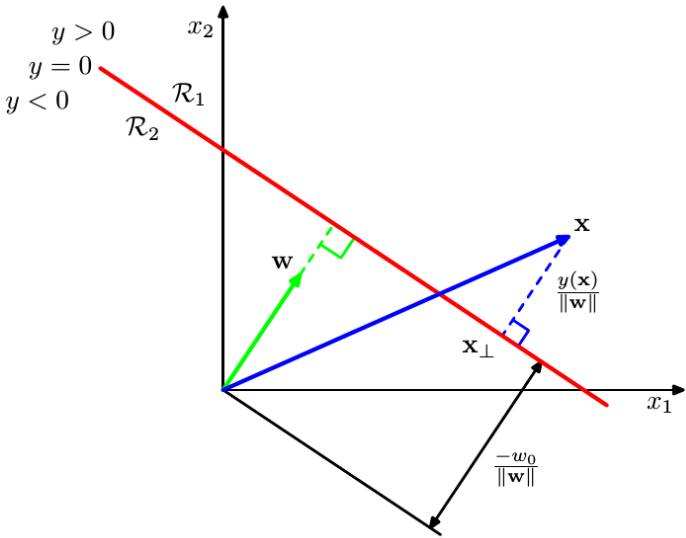
\includegraphics[width=0.35\linewidth]{images/2c.png}
    \caption{Two-class decision problem boundaries}
\end{figure}

\paragraph*{Multiple-class problem}
In multiple class problems with $K$ classes, various encoding methods can be employed:
\begin{itemize}
    \item \textit{One versus the rest}: this approach involves using $K-1$ binary classifiers, where each classifier distinguishes between one class ($C_i$) and the rest of the classes.
        However, this method introduces ambiguity since there may be regions mapped to multiple classes.
    \item \textit{One versus one}: this method utilizes $\frac{K(K-1)}{2}$ binary classifiers, where each classifier discriminates between pairs of classes $C_i$ and $C_j$. 
        Similar to the one versus the rest approach, this method also suffers from ambiguity.
\end{itemize}
One solution to mitigate the ambiguity in multi-class classification is to employ $K$ linear discriminant functions:
\[y_k(\textbf{x})=\textbf{x}^T\textbf{w}_k+w_{k0} \qquad k=1,\dots,K\]
In this approach, an input vector $\textbf{x}$ is assigned to class $C_k$ if $y_k>y_j$ for all $j \neq k$. 
This method ensures that the decision boundaries are singly connected and convex.






\paragraph*{Linear basis function models}
Up to this point, we have focused on models operating within the input space.
However, we can enhance these models by incorporating a fixed set of basis functions $\boldsymbol{\phi}(\textbf{x})$. 
Essentially, this involves applying a non-linear transformation to map the input space into a feature space. 
Consequently, decision boundaries that are linear within the feature space would correspond to nonlinear boundaries within the input space.
This extension enables the application of linear classification models to problems where samples are not linearly separable.

\paragraph*{Ordinary Least Squares}
Let's consider a $K$-class problem using a $1$-of-$K$ encoding for the target. 
Each class is modeled with a linear function:
\[y_k(\textbf{x})=\textbf{x}^T\textbf{w}_k+w_{k0} \qquad k=1,\dots,K\]
In matrix notation, this can be expressed as:
\[\textbf{y}(\textbf{x})=\tilde{\textbf{W}}^T\tilde{\textbf{x}}\]
Given a dataset $\mathcal{D}=\left\{ \textbf{x}_i, \textbf{t}_i  \right\}$ where $i=1,\dots,N$, we can utilize the Least Squares method to determine the optimal value of $\tilde{\textbf{W}}$, resulting in:
\[\tilde{\textbf{W}}=\left(\tilde{\textbf{X}}^T\tilde{\textbf{X}}\right)\tilde{\textbf{X}}^T\tilde{\textbf{T}}\]
In this setup, any new sample $\tilde{\textbf{x}}^T_{new}$ is assigned to class $C_k$ if $t_k>t_j$ for all $j$, where $t_k$ represents the $k$-th component of the model output computed as $t_k=\tilde{\textbf{x}}^T\tilde{\textbf{w}}_k$. 
The primary challenge with employing ordinary Least Squares in classification is that the resulting decision boundaries between regions can vary significantly based on the distribution of the data. 
This method may yield effective or suboptimal boundaries depending on the characteristics of the dataset.





\paragraph*{Perceptron}
To address the issue of poor boundaries, one approach is to utilize a model known as the perceptron. 
Proposed by Rosenblatt in 1958, the perceptron is a linear discriminant model designed specifically for two-class problems, with class encoding as $\{-1,1\}$. 
The perceptron model is defined as:
\[f(\textbf{x},\textbf{w})=\begin{cases}
    +1 \qquad \text{if } \textbf{x}^T\textbf{w}+w_0 \geq 0 \\
    -1 \qquad \text{otherwise}
\end{cases}\]
The perceptron algorithm aims to determine a decision surface, also known as a separating hyperplane, by minimizing the distance of misclassified samples to the boundary. 
This minimization of the loss function can be achieved using stochastic gradient descent.
Although simpler loss functions could theoretically be used, they are often more complex to minimize in practice. 
Therefore, stochastic gradient descent is commonly employed for optimization in perceptron learning.

The perceptron criterion is expressed as:
\[L_P(\textbf{w})=-\sum_{n \in \mathcal{M}}\textbf{w}^T\boldsymbol{\phi}(\textbf{x}_n)t_n\]
Here, correctly classified samples do not contribute to $L$, and each misclassified sample $\textbf{x}_i \in \mathcal{M}$ contributes as $\textbf{w}^T\boldsymbol{\phi}(\textbf{x}_n)t_n$. 

Minimizing $L_P$ is achieved using stochastic gradient descent:
\[\textbf{w}^{(k+1)}=\textbf{w}^{(k)}-\alpha\nabla L_P(\textbf{w})=\textbf{w}^{(k)}+\alpha\boldsymbol{\phi}(\textbf{x}_n)t_n\]
Since the scale of $\textbf{w}$ does not affect the perceptron function, the learning rate $\alpha$ is often set to $1$. 
The perceptron algorithm takes a dataset $\mathcal{D}=\left\{ \textbf{x}_i,\textbf{t}_i  \right\}$ where $i=1,\dots,N$. 
\begin{algorithm}[H]
    \caption{Perceptron}
        \begin{algorithmic}[1]
            \State Initialize $\textbf{w}_0$
            \State $k = 0$
            \Repeat
                \State $k = k+1$
                \State $n = k \mod N$
                \If{$\hat{t}_n \neq t_n$}
                    \State $\textbf{w}_{k+1} = \textbf{w}_k + \boldsymbol{\phi}(\textbf{X}_n)t_n$
                \EndIf
            \Until{convergence}
        \end{algorithmic}
\end{algorithm}
\begin{theorem}[Perceptron convergence]
    If the training dataset is linearly separable in the feature space $\boldsymbol{\Phi}$, then the perceptron learning algorithm is guaranteed to find an exact solution in a finite number of steps.
\end{theorem}
Several steps may be necessary, making it challenging to distinguish between non-separable problems and slowly converging ones. 
If multiple solutions exist, the one obtained by the algorithm depends on the parameter initialization and the order of updates.










\subsection{Probabilistic discriminative approaches}
In a discriminative approach, we model the conditioned class probability directly:
\[\Pr(C_1|\boldsymbol{\phi})=\dfrac{1}{1+e^{-\textbf{w}^T\boldsymbol{\phi}}}=\sigma(\textbf{w}^T\boldsymbol{\phi})\]
This model is commonly referred to as logistic regression.

\paragraph*{Maximum Likelihood}
Given a dataset $\mathcal{D}=\left\{ \textbf{x}_i,t_i \right\}$, where $i=1,\dots,N$ and $t_i \in \{0,1\}$, we aim to maximize the likelihood.
We model the likelihood of a single sample using a Bernoulli distribution, employing the logistic regression model for conditioned class probability:
\[\Pr(t_n|\textbf{x}_n,\textbf{w})=y_n^{t_n}{\left( 1-y_n \right)}^{1-t_n} \qquad y_n=\sigma(\textbf{w}^T\boldsymbol{\phi}_n)\]
Assuming independent sampling of data in $\mathcal{D}$, we have:
\[\Pr(\textbf{t}|\textbf{X},\textbf{w})=\prod_{n=1}^N y_n^{t_n}{\left( 1-y_n \right)}^{(1-t_n)} \qquad y_n=\sigma(\textbf{w}^T\boldsymbol{\phi}_n)\]
The negative log-likelihood (also known as cross-entropy error function) serves as a convenient loss function to minimize:
\[L(\textbf{w})=-\ln \Pr(\textbf{t}|\textbf{X},\textbf{w})=-\sum_{n=1}^N \left( t_n\ln y_n +(1-t_n) \ln (1-y_n) \right) = \sum_{n=1}^N L_n\]
The derivative of $L$ yields the gradient of the loss function:
\[\nabla L(\textbf{w})=\sum_{n=1}^N\left( y_n-t_n \right) \boldsymbol{\phi}_n\]
Due to the nonlinearity of the logistic regression function, a closed-form solution is not feasible. 
Nevertheless, the error function is convex, allowing for gradient-based optimization (even in an online learning setting).

\paragraph*{Multi class logistic regression}
In multi class problems, $\Pr(C_k|\boldsymbol{\phi})$ is modeled by applying a softmax transformation to the output of $K$ linear functions (one for each class):
\[\Pr(C_k|\boldsymbol{\phi})=y_k(\boldsymbol{\phi})=\dfrac{e^{\textbf{w}_k^T\boldsymbol{\phi}}}{\sum_j e^{\textbf{w}_j^T\boldsymbol{\phi}}}\]
Similar to the two-class logistic regression and assuming $1$-of-$K$  encoding for the target, we compute the likelihood as:
\[\Pr(\textbf{T}|\boldsymbol{\Phi},\textbf{w}_1,\dots,\textbf{w}_K)=\prod_{n=1}^N \left( \prod_{k=1}^K \Pr{(C_k|\boldsymbol{\phi}_n)}^{t_n k} \right)=\prod_{n=1}^N \left( \prod_{k=1}^K y^{t_n k}_{nk} \right)\]
As in the two-class problem, we minimize the cross-entropy error function:
\[L(\textbf{w}_1,\dots,\textbf{w}_K)=-\ln \Pr(\textbf{T}|\boldsymbol{\Phi},\textbf{w}_1,\dots,\textbf{w}_K)=-\sum_{n=1}^N \left(\sum_{k=1}^K t_{nk}\ln y_{nk} \right)\]
Then, we compute the gradient for each weight vector:
\[\nabla L_{\textbf{w}_j}(\textbf{w}_1,\dots,\textbf{w}_K)=\sum_{n=1}^N\left( y_{nj}-t_{nj} \right) \boldsymbol{\phi}_n\]

\paragraph*{Perceptron}
Replacing the logistic function with a step function in logistic regression yields the same updating rule as the perceptron algorithm.